% Options for packages loaded elsewhere
\PassOptionsToPackage{unicode}{hyperref}
\PassOptionsToPackage{hyphens}{url}
%
\documentclass[
]{article}
\usepackage{lmodern}
\usepackage{amssymb,amsmath}
\usepackage{ifxetex,ifluatex}
\ifnum 0\ifxetex 1\fi\ifluatex 1\fi=0 % if pdftex
  \usepackage[T1]{fontenc}
  \usepackage[utf8]{inputenc}
  \usepackage{textcomp} % provide euro and other symbols
\else % if luatex or xetex
  \usepackage{unicode-math}
  \defaultfontfeatures{Scale=MatchLowercase}
  \defaultfontfeatures[\rmfamily]{Ligatures=TeX,Scale=1}
\fi
% Use upquote if available, for straight quotes in verbatim environments
\IfFileExists{upquote.sty}{\usepackage{upquote}}{}
\IfFileExists{microtype.sty}{% use microtype if available
  \usepackage[]{microtype}
  \UseMicrotypeSet[protrusion]{basicmath} % disable protrusion for tt fonts
}{}
\makeatletter
\@ifundefined{KOMAClassName}{% if non-KOMA class
  \IfFileExists{parskip.sty}{%
    \usepackage{parskip}
  }{% else
    \setlength{\parindent}{0pt}
    \setlength{\parskip}{6pt plus 2pt minus 1pt}}
}{% if KOMA class
  \KOMAoptions{parskip=half}}
\makeatother
\usepackage{xcolor}
\IfFileExists{xurl.sty}{\usepackage{xurl}}{} % add URL line breaks if available
\IfFileExists{bookmark.sty}{\usepackage{bookmark}}{\usepackage{hyperref}}
\hypersetup{
  hidelinks,
  pdfcreator={LaTeX via pandoc}}
\urlstyle{same} % disable monospaced font for URLs
\usepackage[margin=1in]{geometry}
\usepackage{graphicx,grffile}
\makeatletter
\def\maxwidth{\ifdim\Gin@nat@width>\linewidth\linewidth\else\Gin@nat@width\fi}
\def\maxheight{\ifdim\Gin@nat@height>\textheight\textheight\else\Gin@nat@height\fi}
\makeatother
% Scale images if necessary, so that they will not overflow the page
% margins by default, and it is still possible to overwrite the defaults
% using explicit options in \includegraphics[width, height, ...]{}
\setkeys{Gin}{width=\maxwidth,height=\maxheight,keepaspectratio}
% Set default figure placement to htbp
\makeatletter
\def\fps@figure{htbp}
\makeatother
\setlength{\emergencystretch}{3em} % prevent overfull lines
\providecommand{\tightlist}{%
  \setlength{\itemsep}{0pt}\setlength{\parskip}{0pt}}
\setcounter{secnumdepth}{-\maxdimen} % remove section numbering

\author{}
\date{\vspace{-2.5em}}

\begin{document}

\textbf{Recurrent neural networks}, or RNNs are a special family of
neural networks which were delevoped for modeling \emph{sequential
data}. They process a sequence of values \(x^{(1)}, ..., x^{(t)}\) by
going through its elements one by one and capturing information based on
the previous elements. This information is stored in \textbf{hidden
states} \(h^{(t)}\) as memory of the network. Core idea is rather
simple: we start with a zero vector as a hidden state (because there is
no memory yet), process the current state at time \(t\) and the output
from the previous hidden state, and give the result as an input to the
next iteration.

Basically, a simple RNN is a for-loop that reuses the values which were
calculated in the previous iteration. The total output is a
\emph{tensor} with shape {[}time\_steps, output\_features{]}, where each
time step contains the output of the loop at time \(t\).

\begin{figure}

{\centering 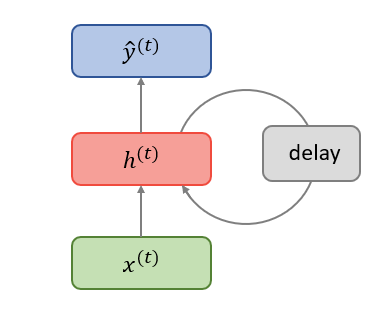
\includegraphics[width=0.3\linewidth]{C:/Users/maria/Documents/LMU/SEMINAR NLP/seminar_nlp_ss20//figures/01-02-rnns-and-their-applications-in-nlp/01_intro_folded_graph} 

}

\caption{Circuit diagram of RNN.}\label{fig:pressure}
\end{figure}

One particular reason why recurrent networks became such a powerful
technique in processing sequential data is the \textbf{parameter
sharing}. Weight matrices for input features remain the same through the
loop and are used repeatedly which makes RNNs extremely convenient to
work with sequential data because the model size does not grow for
longer inputs. In particular, parameter sharing allows application of
the models to inputs of different length and enables generalization
across different positions in time.

As each part of the output is a function of the previous parts of the
output, back-propagation for the RNNs requires recursive computations of
the gradient. The so-called \textbf{back-propagation in time} procedure
is rather simple in theory and allows for the RNNs to access information
from many steps back. In practice though, RNNs in their simple form are
subject to two big problems: \textbf{exploading and vanishing
gradients}. As we compute gradients recursively, they may become either
very small or very large which leads to a complete loss of information
about long-term dependencies. To avoid these problems, \textbf{gated
RNNs} were developed which accumulate information about specific
features over a long duration. We will have a look at two types of gated
RNNs which are widely used in modern Natural Language Processing:
\emph{LSTM} and \emph{GRU}.

Over last couple of years, various extentions of RNNs were developed
which resulted in their wide application in different fields of Natural
Language Processing. Beside classical tasks as document classification
and sentiment analysis more complicated challenges such as machine
translation, part-of-speech tagging or speech recognition can be solved
nowadays with help of cutting-edge versions of RNNs. An overview of
these versions and their applications will be provided in the last part
of Chapter 1.2.

\end{document}
